\documentclass[12pt,a4paper]{report}

\usepackage{config/uepThesis}

\addbibresource{bibliografia.bib}

%%%%% STRONA TYTUŁOWA PRACY %%%%%%%%%%%%%%%%%%%%%%%%%%
%%%%% NIEZBĘDNA KONFIGURACJA DO WYGENEROWANIA STRONY TYTUŁOWEJ %%%%%

\usepackage{stronaTytulowa/uepTitle}

%%% TYTUŁ PRACY PO POLSKU %%%
\title{Zmiana struktury kosztów jako środek do modyfikacji modelu biznesowego}

%%% TYTUŁ PRACY PO ANGIELSKU %%%
\titleEN{Changing the cost structure as a means to modify the business model}

%%% RODZAJ PRACY %%% proszę od-komentować odpowiedni rodzaj pracy
\thesisType{Praca licencjacka}
%\thesisType{Praca inżynierska}
%\thesisType{Praca magisterska}

%%% AUTOR %%%
\author{Anna Kowalska}

%%% PROMOTOR %%%
\supervisor{dr M. Nowak}

%%% KIERUNEK %%%
\major{Zarządzanie}

%%%%%%%%%%%%%%%%%%%%%%%%%%%%%%%%%%%%%%%%%%%%%

\begin{document}

\maketitle

% TREŚCI PRACY %
\section{Zarządzanie}

Zarządzanie – ogólny zakres działań, procesów i decyzji, których zastosowanie w odniesieniu do zasobów, osób, kapitału lub organizacji ma zapewnić warunki do efektywnego ich funkcjonowania prowadzącego do osiągnięcia postawionych celów. \cite{French2010, Shotton1999, Shotton1989} 

\[
\sqrt{x^2+1}
\]

Od początku XX wieku, odkąd zarządzanie próbowano oprzeć na naukowych podstawach, aż do lat 60. XX wieku zarządzanie pojmowane było jako działanie kierownicze, obejmujące następujące sekwencje postępowania: planowanie, organizowanie, decydowanie, motywowanie i kontrolowanie, nazywane klasycznymi funkcjami zarządzania. \cite[123--126]{Lassen2006}

Klasyczne funkcje zarządzania wyróżnił pierwszy „klasyk” zarządzania Henri Fayol. Jednakże paradygmat zarządzania zmienił się od tego czasu radykalnie, więc warto powrócić do starszej, bardziej ogólnej definicji \textcite[610]{Porter1981} twierdz: zarządzanie to sztuka bądź praktyka rozumnego stosowania środków dla osiągnięcia wyznaczonych celów. \cite[25-28]{klimczak2007effect}

\subsection{Zarządzanie w gospodarce}

W odniesieniu do organizacji gospodarczych zamiast słowa zarządzanie używa się czasem terminu administracja biznesu (ang. Business Administration). Zadanie administracji biznesu ujmuje krótkie określenie: „Administracja biznesu ma zapewnić, aby zostało zrobione to, co ma być zrobione”. Administracja biznesu jest dyscypliną akademicką, a szereg uniwersytetów i szkół biznesu nadaje stopień magistra z tej dyscypliny (Master of Business Administration, w skrócie MBA). \cite{Lassen2006}

\begin{figure}[!ht]
	\centering
	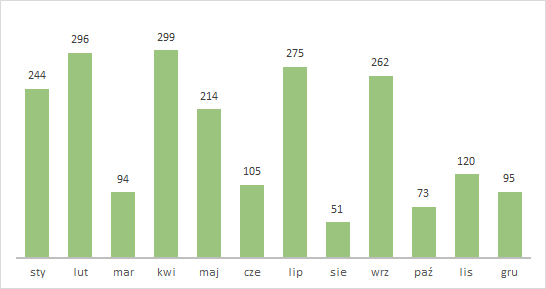
\includegraphics[width=\textwidth]{rozdzial1/wykres.png}
	\caption{{\bfseries Zmiana wartości w czasie}
	\\ \footnotesize{Źródło: \protect\cite{Shotton1999}}}
	\label{fig:wykres}
\end{figure}

\subsection{Zarządzanie w gospodarce}

W odniesieniu do organizacji gospodarczych zamiast słowa zarządzanie używa się czasem terminu administracja biznesu (ang. Business Administration). Zadanie administracji biznesu ujmuje krótkie określenie: „Administracja biznesu ma zapewnić, aby zostało zrobione to, co ma być zrobione”. Administracja biznesu jest dyscypliną akademicką, a szereg uniwersytetów i szkół biznesu nadaje stopień magistra z tej dyscypliny (Master of Business Administration, w skrócie MBA). \cite{Lassen2006}
\clearpage %dodajemy w celu rozpoczęcia kolejnego rozdziału od nowej strony
\section{Badania}

Jedna z metod badań społecznych, w której do zbierania informacji od respondentów wykorzystuje się wystandaryzowany kwestionariusz. \cite{French2010a}

Dla ustalenia badanej populacji konsumentów \cite{nbp2012} stosuje się dobór losowy, gdy niewielka jest ich liczba i nieznana ich struktura, dobór losowy systematyczny \cite{nbp2012}, gdy dostępna jest lista całej populacji oraz dobór losowy \cite{systems2001} warstwowy dla uzyskania bardziej dokładnych wyników charakteryzujących badanych. \cite{Shotton2000, French2010, Shotton2010, Shotton1989, French2010a, Shotton1999}

Stan negatywnych emocji i frustracji w niektórych kręgach akademickiej makroekonomii \textcite[25]{krugman2009} najlepiej oddaje skrajna wypowiedź Krugmana \parencite*{krugman2009}: „Większość z tego, co stworzono w ramach makroekonomii w ciągu ostatnich 30 lat okazało się w najlepszym razie bezużyteczne lub w najgorszym razie szkodliwe” \citepage[20]{krugman2009}.

\begin{table}[h!]
	\begin{center}
		\caption{{\bfseries Wyniki badań}}
		\label{tab:table1}
		\begin{tabular}{l|c|r} % <-- Alignments: 1st column left, 2nd middle and 3rd right, with vertical lines in between
			\textbf{Value 1} & \textbf{Value 2} & \textbf{Value 3}\\
			$\alpha$ & $\beta$ & $\gamma$ \\
			\hline
			1 & 1110.1 & a\\
			2 & 10.1 & b\\
			3 & 23.113231 & c\\
		\end{tabular}
	\end{center}
	\begin{center}
	    \footnotesize{Źródło: \protect\cite{Shotton1999}}
	\end{center}
\end{table}
% tu proszę wstawiać kolejne elementy pracy np. rozdział 3 itd.
% KONIEC TREŚCI PRACY %

\printbibliography

\listoffigures

\listoftables

\end{document}